\documentclass[aspectratio=43]{beamer}
\usepackage[english]{babel}
\usepackage{amsthm}
\usepackage{amsfonts}
\usepackage{amsmath}
\usepackage{amssymb}
\usepackage{mathtools}
% \usepackage{bbm}
\usepackage{pgfplots}
\usepackage{tikz}
% \usepackage{physics}
\usepackage{calligra}
\usepackage{csquotes}
% \usepackage{tensor}
\usepackage[thicklines]{cancel}
\usepackage{tcolorbox}
\usepackage{pstricks}
\usepackage{todonotes}
\usepackage[backend=biber, sorting=nty, citestyle=numeric-comp]{biblatex} %Custom bibliography
    \addbibresource{bib.bib} %Load references


\DeclareMathAlphabet{\mathcalligra}{T1}{calligra}{m}{n}
\DeclareFontShape{T1}{calligra}{m}{n}{<->s*[2.2]callig15}{}
\newcommand{\scriptr}{\mathcalligra{r}\,}
\newcommand{\boldscriptr}{\pmb{\mathcalligra{r}}\,}
\def\rc{\scriptr}
\def\brc{\boldscriptr}
\def\hrc{\hat\brc}
\newcommand{\ie}{\emph{i.e.}} %id est
\newcommand{\eg}{\emph{e.g.}} %exempli gratia
\newcommand{\rtd}[1]{\ensuremath{\left\lfloor #1 \right\rfloor}}
\newcommand{\dirac}[1]{\ensuremath{\delta \left( #1 \right)}}
\newcommand{\diract}[1]{\ensuremath{\delta^3 \left( #1 \right)}}
\newcommand{\e}{\ensuremath{\epsilon_0}}
\newcommand{\m}{\ensuremath{\mu_0}}
\newcommand{\V}{\ensuremath{\mathcal{V}}}
\newcommand{\prnt}[1]{\ensuremath{\left(#1\right)}} %parentheses
\newcommand{\colch}[1]{\ensuremath{\left[#1\right]}} %square brackets
\newcommand{\chave}[1]{\ensuremath{\left\{#1\right\}}}  %curly brackets
\newcommand\eqdef{\stackrel{\mathclap{\normalfont \tiny\mbox{\textrm{def}}}}{=}}
\useoutertheme{infolines}
\useinnertheme{rectangles}
\usefonttheme{professionalfonts}


\definecolor{blue2}{HTML}{045FB4}
\definecolor{green2}{HTML}{46C235}
\definecolor{red2}{HTML}{EE4848}
\definecolor{violet2}{HTML}{A647E5}
\definecolor{orange2}{HTML}{FF7425}
\definecolor{darkred}{HTML}{5C2020}
\definecolor{gray}{HTML}{303030}
\definecolor{yellow}{HTML}{f0be52}
\definecolor{lightdarkgold}{HTML}{EEBC1D}

\renewcommand{\CancelColor}{\color{darkred}}

\makeatletter
\newcommand{\mybox}[1]{%
  \setbox0=\hbox{#1}%
  \setlength{\@tempdima}{\dimexpr\wd0+13pt}%
  \begin{tcolorbox}[colback=darkred,colframe=darkred,boxrule=0.5pt,arc=4pt,
      left=6pt,right=6pt,top=6pt,bottom=6pt,boxsep=0pt,width=\@tempdima]
    \textcolor{yellow}{#1}
  \end{tcolorbox}
}
\makeatother


\pgfplotsset{my style/.append style={axis x line=middle, axis y line=
middle, xlabel={$x$}, ylabel={$y$}, axis equal }}


\usecolortheme[named=darkred]{structure}
\usecolortheme{sidebartab}
\usecolortheme{orchid}
\usecolortheme{whale}
\setbeamercolor{titlelike}{parent=structure, bg=structure, fg=white}
\setbeamercolor{section in toc}{fg= white}
\setbeamercolor{subsection in toc}{fg= white}
%\setbeamercolor*{sidebar}{fg=red2,bg=gray!15!white}

\setbeamercolor{item projected}{bg=yellow, fg = darkred}
\setbeamertemplate{enumerate items}[default]
\setbeamertemplate{navigation symbols}{}
\setbeamercolor{local structure}{fg=yellow}

\setbeamercolor{alerted text}{fg=white}
\setbeamercolor{block title}{bg = blue2}
\setbeamercolor{block title alerted}{bg=red2}
\setbeamercolor{block title example}{bg=green2}
\setbeamercolor{background canvas}{bg=gray}
\setbeamercolor{normal text}{bg=gray,fg=white}


\setbeamertemplate{footline}
        {
      \leavevmode%
      \hbox{%
      \begin{beamercolorbox}[wd=.333333\paperwidth,ht=2.25ex,dp=1ex,center]{author in head/foot}%
        \usebeamerfont{author in head/foot}\insertshortauthor~~(\insertshortinstitute)
      \end{beamercolorbox}%
      \begin{beamercolorbox}[wd=.333333\paperwidth,ht=2.25ex,dp=1ex,center]{title in head/foot}%
        \usebeamerfont{title in head/foot}\insertshorttitle
      \end{beamercolorbox}%
      \begin{beamercolorbox}[wd=.333333\paperwidth,ht=2.25ex,dp=1ex,center]{date in head/foot}%
        \usebeamerfont{date in head/foot}\insertshortdate{}%\hspace*{2em}

    %#turning the next line into a comment, erases the frame numbers
        %\insertframenumber{} / \inserttotalframenumber\hspace*{2ex} 

      \end{beamercolorbox}}%
      \vskip0pt%
    }


\setbeamertemplate{blocks}[rectangle]
\setbeamercovered{dynamic}




%\setbeamercolor{author}{fg=yellow}
%\setbeamercolor{title}{fg = yellow}
%\setbeamerfont{title}{size=\Large, series=\bfseries}
%\setbeamerfont{author}{size=\footnotesize}
%\setbeamerfont{date}{size=\small}


\setbeamertemplate{section page}
{
	\begin{centering}
		\begin{beamercolorbox}[sep=27pt,center]{part title}
			\usebeamerfont{section title}\insertsection\par
			\usebeamerfont{subsection title}\insertsubsection\par
		\end{beamercolorbox}
	\end{centering}
}





%\setbeamertemplate{subsection page}
%{
%	\begin{centering}
%		\begin{beamercolorbox}[sep=12pt,center]{part title}
%			\usebeamerfont{subsection title}\insertsubsection\par
%		\end{beamercolorbox}
%	\end{centering}
%}

\newcommand{\hlight}[1]{\colorbox{violet!50}{#1}}
\newcommand{\hlighta}[1]{\colorbox{darkred!50}{#1}}

\title{Eingangsvorlesung} %->->->->-> Check hyperref title <-<-<-<-<-
\subtitle{Administrives und Vorschau}
\author[Lechner/Rumori]{\textcolor{yellow}{Patrik Lechner, Martin Rumori}}
\institute[IC\textbackslash M/T]{
    % \textcolor{white}{Institute of Mathematics}%
    \\%
    \textcolor{white}{FH St.Pölten}%
} %You can change the Institution if you are from somewhere else
% \date{Feb. 30, 2142}
%\logo{\includegraphics[width= 0.05\textwidth]{images/logo.png}}

\begin{document}
    
    \frame{\titlepage}
    
    \begin{frame}{Inhalt}
        \tableofcontents
    \end{frame}
    %!TEX root = ../main.tex
\section{Idee der LV}
 \frame{\sectionpage}

\begin{frame}{Ziele}
Das Ziel der LV ist es, in einer kollaborativen Arbeitsweise eine interaktive Installation umzusetzen.

\begin{itemize}
    \item \textcolor{white}{Aneignung von Wissen und Fertigkeiten in Theorie und Praxis}
    \item \textcolor{white}{Koordination von Expertise}
    \item \textcolor{red2}{Umsetzung einer Projektidee}
\end{itemize}
    
\end{frame}

\begin{frame}{Was für ein Projekt?}
Beispiele später, Grundzüge:

\begin{itemize}
    \item Interaktive Aspekte (daher Sensorik)
    \item Audio-Aspekte (Sonifikation, Sound-Design)
    \item Video-Aspekte (Visualisierung)
\end{itemize}

\end{frame}

% \begin{frame}{Blocks}
% \begin{block}{begin block}
% There's a block
% \end{block}

% \begin{alertblock}{begin alertblock}
%     there's a alert block 
% \end{alertblock}

% \begin{exampleblock}{begin example block}
% here comes example
% \end{exampleblock} 

% \end{frame}


% \begin{frame}{Blocks}
    
% \begin{theorem}
%     Here comes a theorem
% \end{theorem}

% \begin{proof}
%     Here comes the proof
% \end{proof}


    
% \end{frame}
    
    %!TEX root = ../main.tex

\section{Administratives}
 \frame{\sectionpage}

\begin{frame}{Benotung}

 
\begin{table}[]
\begin{tabular}{l|l}
Zwischen Prüfungen & End Projekt \\ \hline
30\%                & 70\%       
\end{tabular}
\end{table}


\end{frame}


\begin{frame}{Notenschlüssel}

 
\begin{table}[]
\begin{tabular}{l|l}
Punkte & Note \\ \hline
0-49   & 5    \\
50-60  & 4    \\
60-80  & 3    \\
80-90  & 2    \\
90-100 & 1   
\end{tabular}
\end{table}

\end{frame}


\begin{frame}{Tasks / Important Dates}
\todo[inline]{check dates}
\begin{table}[]
\begin{tabular}{l|l|l}
\emph{Was}   &  \emph{Wie}             &	\emph{Wann}	\\ \hline
Gruppen Einteilung   & Am Ecampus              &		\\  
Zwischenprüfungen        & 5-10 min Ecampus              &	Laufend	\\
Projekt Pitch        & Informelles Gespräch              &	Anfang April	\\
Project Support      & Frei Abeiten in UE              &	Mai/Juni	\\
Project Presentation & 15 min Presentation & Prüfungswoche \\
Project Doku + Submission & Showreel Eintrag & Prüfungswoche
\end{tabular}
\end{table}

\end{frame}

    %!TEX root = ../main.tex
\section{Inhalte der LV}
 \frame{\sectionpage}

    %!TEX root = ../main.tex
\section{Projekt Beispiele}
 \frame{\sectionpage}

    %!TEX root = ../main.tex
\section{Inputs/Sensoren}
 \frame{\sectionpage}

\begin{frame}{Kameras}

Wir verwenden hauptsaechlich webcams da die einbindung in einen realtime kontext am einfachsten/gängigsten ist.

\begin{itemize}
	\item 'Übliche' Webcams
	\item Hoeher qualitative Kameras mit echtzeit output
	\item Analoge Cams + capture Karten
	\item Stereo Kamera setups
	\item 360 Grad Kameras
	\item ...
\end{itemize}

\end{frame}


\begin{frame}{Mikrophone}
\begin{itemize}
	\item 'Übliche' Mikrophone
	\item piezo mikrophone (Körperschall)
	\item mehrkanal setups (zb. mic arrays)
\end{itemize}
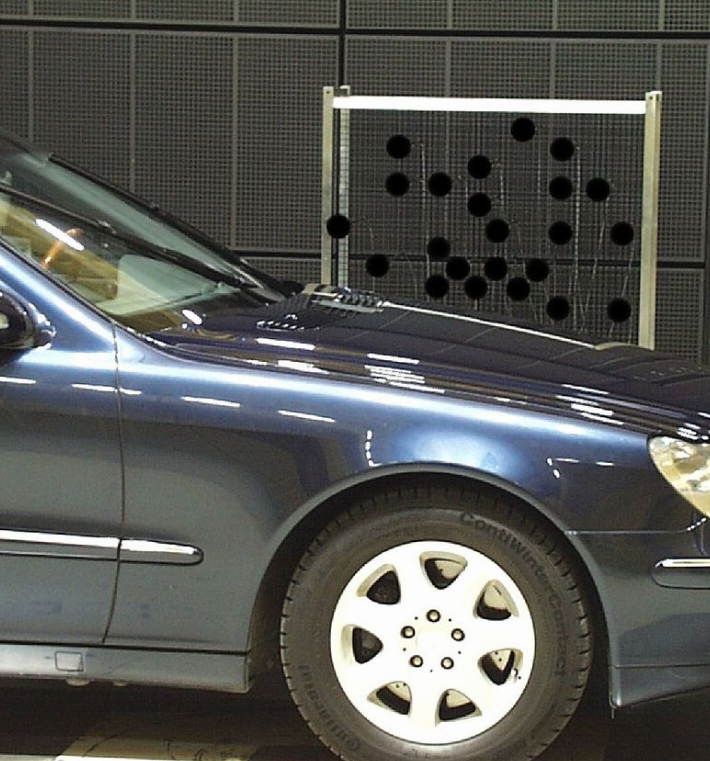
\includegraphics[width=\textwidth]{micarr.png}

\end{frame}


\begin{frame}{3D Cameras}
\begin{itemize}
	\item intel real sense
	\item kinect
	\item nicht vergessen: K.I. benutzen um 3D info zu schätzen. z.B. 'Posenet'.
\end{itemize}
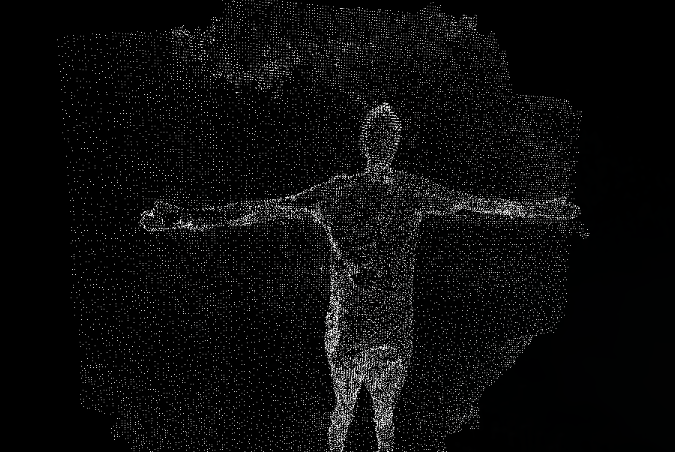
\includegraphics[width=\textwidth]{pcloud.png}
\end{frame}

\begin{frame}{HID (Human Interface devices)}
	\begin{itemize}
		\item Computer keyboard 
		\item Diverse Midi controller
		\item Touchscreens
		\item div. potentiometer (nicht zwangsläufig MIDI)
		\item Eye-tracking
		\item handtracking (-> 'leap motion')
		\item 3d tracking im raum (zb. Vive controller)
		\item ...
	\end{itemize}
% 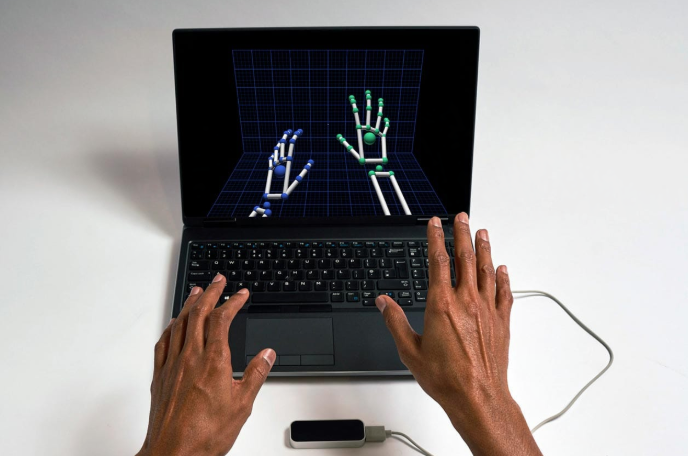
\includegraphics[width=5cm]{leap.png}
\begin{center}
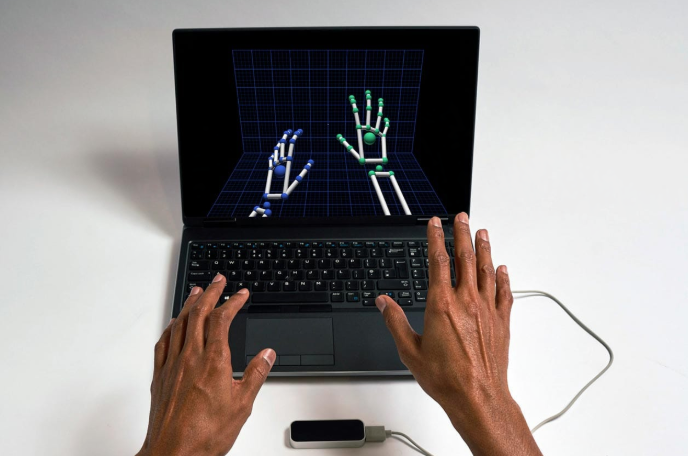
\includegraphics[width=5cm]{leap.png}
\end{center}

\end{frame}


\begin{frame}{Sonstige Sensoren}

\begin{columns}
	\begin{column}{0.5\textwidth}
		\begin{itemize}
		\item Accelerometer
		\item Thermometer
		\item Ultraschall distanzmesser
		\item Photoresistoren
		\item ....
		\end{itemize}
	\end{column}

	\begin{column}{0.5\textwidth}
		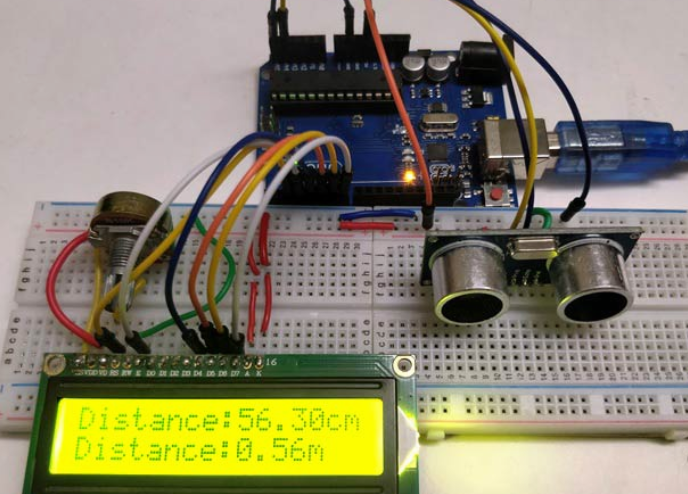
\includegraphics[width=5cm]{dist.png}
	\end{column}

\end{columns}

\end{frame}

\begin{frame}{APIs und open data}
\begin{itemize}
	\item twitter
	\item soundcloud
	\item instagram
	\item telegram bot
	\item open gov data
	\item .....

\end{itemize}
\begin{center}
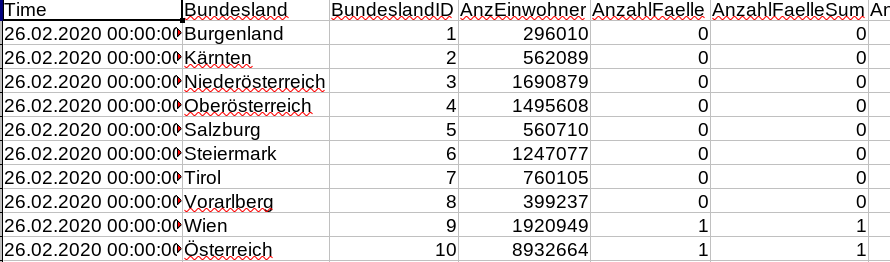
\includegraphics[width=\textwidth]{api.png}
\end{center}


\end{frame}

\section{Outputs/Dispositive}
 \frame{\sectionpage}

\begin{frame}{Screens}

\begin{itemize}
	\item 'Üblicher' Screen
	\item 'Üblicher' Screen + headtracking
	\item multi screen setups
	\item analog screens
	\item ...

\end{itemize}

\begin{center}
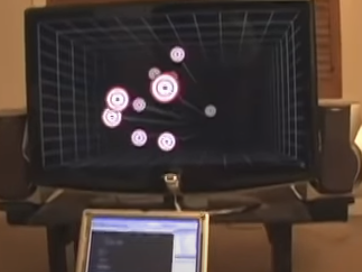
\includegraphics[width=7cm]{screen.png}
\end{center}




\end{frame}


\begin{frame}{Projektoren}
\begin{itemize}
	\item Standard Projektion
	\item 3D Projektion (shutter brillen etc)
	\item 2d/3D Mapping
	\item Räumliche Dispositive (z.B. Fulldome)
	\item 'Hologramme'
\end{itemize}

\begin{center}
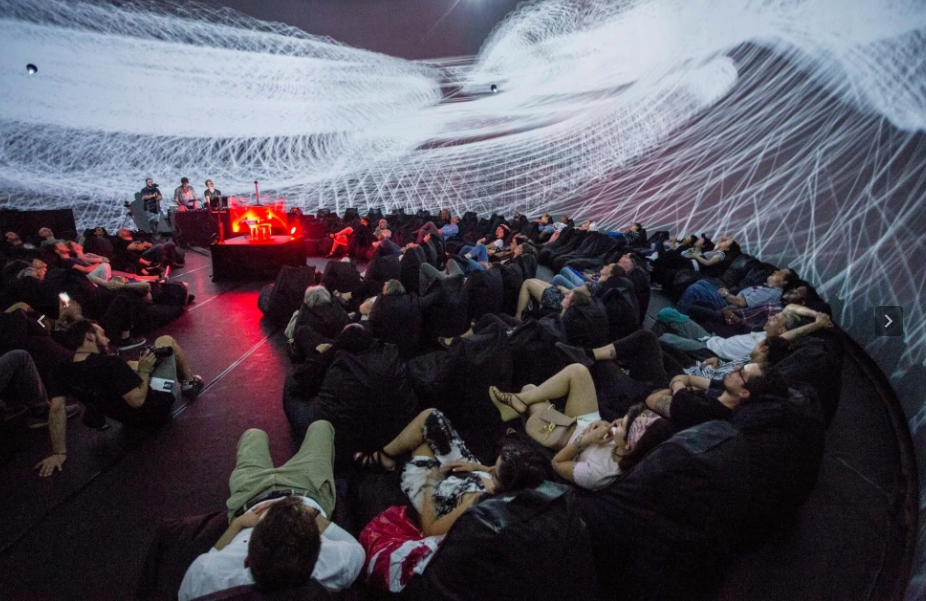
\includegraphics[width=7cm]{dome.png}
\end{center}
\end{frame}


\begin{frame}{Lautsprecher, Kopfhoerer}
\begin{itemize}
	\item "Übliche" Lautsprecher Setups
	\item Kopfhörer (+ headtracking)
	\item Ambisonics u diverse 3D audio verfahren
	\item 'butt shaker'/'butt kicker'
	\item div. körperschall transducer
	\item ultraschall Richtlautsprecher
\end{itemize}

\begin{center}
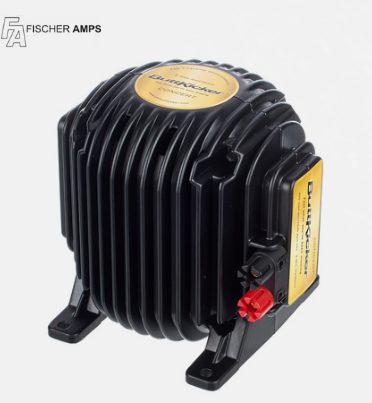
\includegraphics[width=5cm]{butt.png}
\end{center}

\end{frame}

\begin{frame}{Sonstiges}
\begin{itemize}
	\item Professionelle Lichtanlagen (DMX)
	\item Licht, LED strips
	\item Motoren, pumpen etc
\end{itemize}

\begin{center}
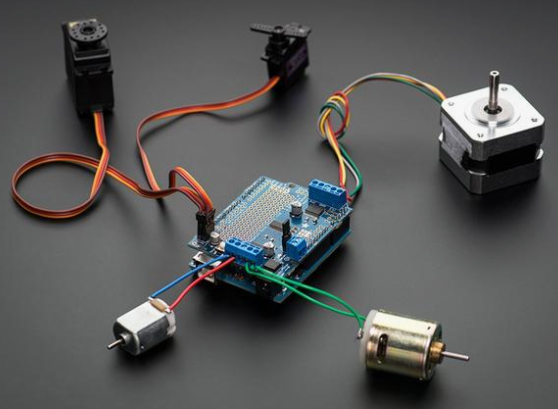
\includegraphics[width=7cm]{motor.png}
\end{center}
\end{frame}


\begin{frame}{APIs}
\begin{itemize}
	\item twitter
	\item instagram
	\item SoundCloud
	\item telegram bot
	\item ...
\end{itemize}

\begin{center}
\begin{figure}

\includegraphics[width=9cm]{bot.png}
\caption{EIn fehlgeschlagener Microsoft Bot entpuppt sich binnen 24h zum Menschhassser.}
\end{figure}
\end{center}


\end{frame}




    
    
    % \section{Equations and Figure}
     
    \frame{\sectionpage}
    
    \begin{frame}{Ordinary Differential Equations}
        \uncover<+->{\begin{equation*}
            \dv{x} y(x) + \frac{1}{CR} y(x) = 0
        \end{equation*}}
        
        \uncover<+->{\begin{equation}
            \dv[2]{x} y(x) + \gamma \dv{x} y(x) + \omega_0^2 y(x) = f(x)
        \end{equation}}
    \end{frame}
    
    \begin{frame}{}
        \uncover<+>{\begin{equation*}
            \dv[2]{x} y(x) + \gamma \dv{x} y(x) + \omega_0^2 y(x) = f(x)
        \end{equation*}}
        \uncover<+>{\[ \Downarrow \]
        \begin{equation*}
            \colch{\dv[2]{x} + \gamma \dv{x} + \omega_0^2} y(x) = f(x)
        \end{equation*}}
        \uncover<+>{\[ \Downarrow \]
        \begin{equation*}
            y(x) = \frac{f(x)}{\dv[2]{x} + \gamma \dv{x} + \omega_0^2}
        \end{equation*}}
    \end{frame}
    
    \begin{frame}{Imagem}
        \centering
        \includegraphics[width = 0.8\textwidth]{images/coke.jpg}\\
        \footnotesize \textcolor{yellow}{Figure:} Some words about the figure here
    \end{frame}
    
 
    \begin{frame}{See how is cool the fourier serie}
        \uncover<+>{\begin{equation*}
            \mathcal{F}[f](\xi) = \hat{f}(\xi) = \frac{1}{\sqrt{2\pi}} \int_{-\infty}^{+\infty} f(x) e^{-i x \xi} \dd{x}
        \end{equation*}}
        \uncover<+>{\begin{equation*}
            \mathcal{F}^{-1}[\hat{f}](x) = f(x) = \frac{1}{\sqrt{2\pi}} \int_{-\infty}^{+\infty} \hat{f}(\xi) e^{i x \xi} \dd{\xi}
        \end{equation*}}
    \end{frame}
    
    \begin{frame}{Quality Control}
        \uncover<+>{\begin{equation*}
            \widehat{(f + \alpha g)}(\xi) = \frac{1}{\sqrt{2\pi}} \int_{-\infty}^{+\infty} \prnt{f(x) + \alpha g(x)} e^{-i x \xi} \dd{x}
        \end{equation*}}
        \uncover<+>{\[ \Downarrow \]
        \begin{equation*}
            \widehat{(f + \alpha g)}(\xi) = \frac{1}{\sqrt{2\pi}} \int_{-\infty}^{+\infty} f(x) e^{-i x \xi} \dd{x} + \frac{\alpha}{\sqrt{2\pi}} \int_{-\infty}^{+\infty} g(x) e^{-i x \xi} \dd{x}
        \end{equation*}}
        \uncover<+>{\[ \Downarrow \]
        \begin{equation*}
            \widehat{(f + \alpha g)}(\xi) = \hat{f}(\xi) + \alpha \hat{g}(\xi)
        \end{equation*}}
    \end{frame}
    
    \begin{frame}{Quality Control}
        \uncover<+>{\begin{equation*}
            \widehat{f'}(\xi) = \frac{1}{\sqrt{2\pi}} \int_{-\infty}^{+\infty} f'(x) e^{-i x \xi} \dd{x}
        \end{equation*}}
        \uncover<+>{\[ \Downarrow \]
        \begin{equation*}
            \widehat{f'}(\xi) = \eval{\frac{f(x) e^{-ix\xi}}{\sqrt{2\pi}}}^{+\infty}_{-\infty} + i\xi \cdot \frac{1}{\sqrt{2\pi}} \int_{-\infty}^{+\infty} f(x) e^{-i x \xi} \dd{x}
        \end{equation*}}
        \uncover<+>{\[ \Downarrow \]
        \begin{equation*}
            \widehat{f'}(\xi) = i\xi \widehat{f}(\xi)
        \end{equation*}}
    \end{frame}
    
    \begin{frame}{Quality Control}
        \centering
        \textcolor{green2}{\huge{The inverse does work}}
        
        \normalsize{for appropriate functions} 
        
        \tiny{and, sometimes, the Fourier Transform of a function is not in the same set as the original function, but let's forget about this since we do not know a decent theory of integration}
    \end{frame} 
    
    % \section{graphs and other tikz}
 \frame{\sectionpage}
 
\begin{frame}{Drawning within tikz}
    \tikzset{every picture/.style={line width=0.75pt}} %set default line width to 0.75pt        

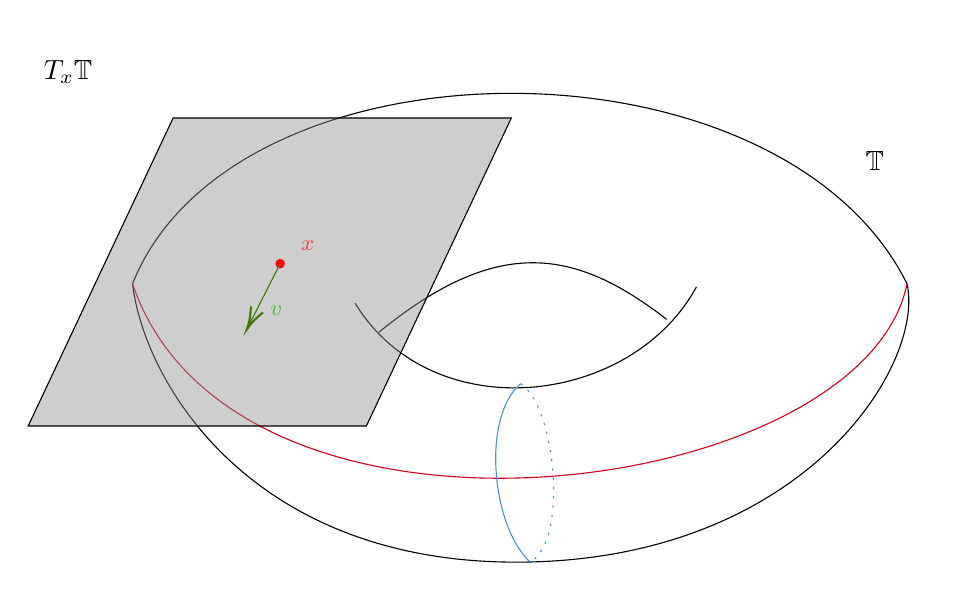
\begin{tikzpicture}[x=0.75pt,y=0.75pt,yscale=-1,xscale=1]
%uncomment if require: \path (0,486); %set diagram left start at 0, and has height of 486

%Curve Lines [id:da9595099437611456] 
\draw    (233.23,183.24) .. controls (252.87,215.34) and (288.86,227.45) .. (323.09,223.22) .. controls (353.65,219.45) and (382.81,202.65) .. (397.65,175.44) ;
%Curve Lines [id:da6932103982097759] 
\draw    (244.67,197.26) .. controls (301.86,150.51) and (339.03,156.74) .. (383.35,191.03) ;
%Curve Lines [id:da7053828945347995] 
\draw    (126,173.88) .. controls (131.72,222.2) and (184.62,311.04) .. (317.59,307.92) .. controls (450.55,304.8) and (507.74,212.85) .. (499.16,173.88) ;
%Curve Lines [id:da583602680611125] 
\draw    (126,173.88) .. controls (174.61,52.32) and (437.68,50.76) .. (499.16,173.88) ;
%Curve Lines [id:da5190289437371578] 
\draw [color={rgb, 255:red, 208; green, 2; blue, 27 }  ,draw opacity=1 ]   (126,173.88) .. controls (175,318) and (478,278) .. (499.16,173.88) ;
%Curve Lines [id:da5494113181101443] 
\draw [color={rgb, 255:red, 74; green, 144; blue, 226 }  ,draw opacity=1 ]   (313,222) .. controls (294,238) and (299,291) .. (317.59,307.92) ;
%Curve Lines [id:da8828117501564781] 
\draw [color={rgb, 255:red, 74; green, 144; blue, 226 }  ,draw opacity=1 ] [dash pattern={on 0.84pt off 2.51pt}]  (313,222) .. controls (330,233) and (336,298) .. (317.59,307.92) ;
%Shape: Parallelogram [id:dp02778297397005436] 
\draw  [fill={rgb, 255:red, 144; green, 144; blue, 144 }  ,fill opacity=0.44 ] (145.57,94) -- (308.5,94) -- (238.68,242.38) -- (75.75,242.38) -- cycle ;
%Shape: Circle [id:dp8371213746664339] 
\draw  [color={rgb, 255:red, 253; green, 1; blue, 1 }  ,draw opacity=1 ][fill={rgb, 255:red, 255; green, 0; blue, 0 }  ,fill opacity=1 ] (195.13,164.19) .. controls (195.13,163.08) and (196.02,162.19) .. (197.13,162.19) .. controls (198.23,162.19) and (199.13,163.08) .. (199.13,164.19) .. controls (199.13,165.29) and (198.23,166.19) .. (197.13,166.19) .. controls (196.02,166.19) and (195.13,165.29) .. (195.13,164.19) -- cycle ;
%Straight Lines [id:da21346648436809335] 
\draw [color={rgb, 255:red, 65; green, 117; blue, 5 }  ,draw opacity=1 ]   (197.13,164.19) -- (181.9,194.22) ;
\draw [shift={(181,196)}, rotate = 296.88] [color={rgb, 255:red, 65; green, 117; blue, 5 }  ,draw opacity=1 ][line width=0.75]    (10.93,-3.29) .. controls (6.95,-1.4) and (3.31,-0.3) .. (0,0) .. controls (3.31,0.3) and (6.95,1.4) .. (10.93,3.29)   ;

% Text Node
\draw (501,122.4) node [anchor=north west][inner sep=0.75pt]    {$\ $};
% Text Node
\draw (478,109) node [anchor=north west][inner sep=0.75pt]   [align=left] {\(\mathbb{T}\)};
% Text Node
\draw (82,65) node [anchor=north west][inner sep=0.75pt]   [align=left] {\(T_x\mathbb{T}\)};
% Text Node
\draw (206,152) node [anchor=north west][inner sep=0.75pt]   [align=left] {\textcolor{red2}{{\footnotesize \(x\)}}};
% Text Node
\draw (191.06,183.09) node [anchor=north west][inner sep=0.75pt]   [align=left] {{\footnotesize \textcolor{green2}{\(v\)}}};

\end{tikzpicture}

    
\end{frame}



\begin{frame}{It's possible plotting graphs with pgfplots and tikz}

\centering
\begin{tikzpicture}
\begin{axis}
\addplot[color=yellow]{exp(x)};
\end{axis}
\end{tikzpicture}
%Here ends the 2D plot

%Here ends the 3D plot

\end{frame}

\begin{frame}{Plotting 3d}
%Here begins the 3D plot
\centering
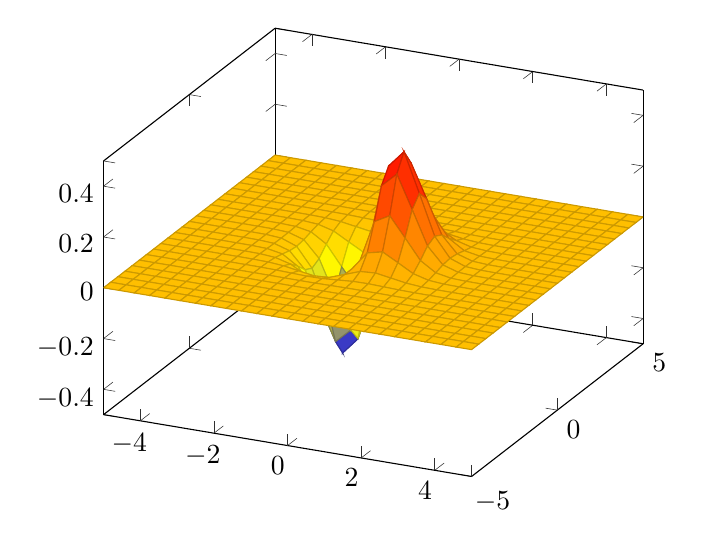
\begin{tikzpicture}
\begin{axis}
\addplot3[
    surf,
]
{exp(-x^2-y^2)*x};
\end{axis}
\end{tikzpicture}
\end{frame}
    
    
 %   \section*{References} %You can remove this if you do not want to use it
 %       \nocite{Djairo} \nocite{PhilPanof} \nocite{Fleming} \nocite{Shankar}
 %       \begin{frame}{References}
 %           \printbibliography
 %       \end{frame}

    \section{}
    \begin{frame}{}
        \centering
            \Huge\bfseries
        \textcolor{yellow}{The End}
    \end{frame}
\end{document}
